\subsection{Automaten}
Es wurde versucht Automaten sowohl möglichst nah an der theoretischen Vorgabe als auch möglichst effizient zu implementieren. Herausgekommen ist dabei folgende Grundimplementation:
\begin{figure}[h]
  \centering
  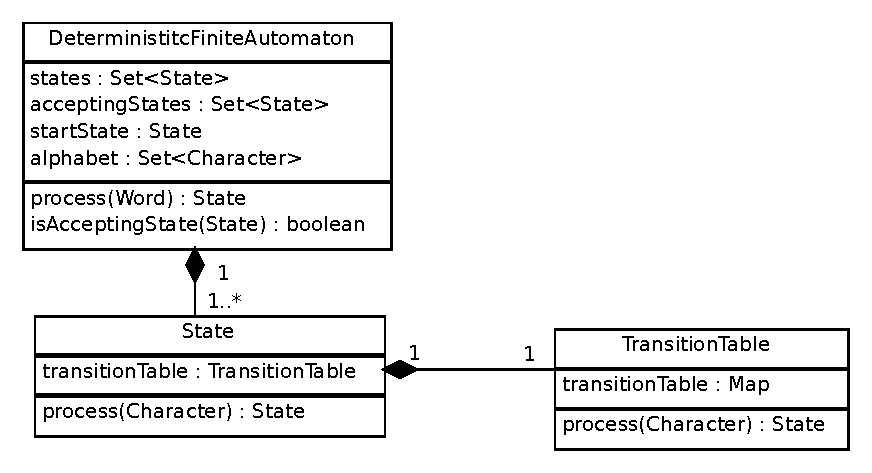
\includegraphics[width=0.5\textwidth]{images/dfa_classdiag_simple.pdf}
  \caption[DFA Klassendiagramm vereinfacht]{DFA Klassendiagramm vereinfacht}
  \label{fig:dfa_classdiag_simple}
\end{figure}

Das Quintupel ($Q$, $\Sigma$, $\delta$, $q0$, $F$) ist darin wie folgt abgebildet:

\begin{table}[h]
  \centering
  \begin{tabular}{ l | l }
    \hline
    $Q$ & Die Menge der Zustände wurde als Set von States implementiert.  \\
    \hline
    $\Sigma$ & Das Alphabet ist ein Array von Zeichen (Character). \\
    \hline
    $\delta$ & Die Übergangsfunktion $\delta$ wird als Map (Zeichen -> Zustand) 
    \\ & auf den einzelnen Zuständen abgebildet. Dies erlaubt uns eine
    \\ & einfache und effiziente Verarbeitung von Eingaben sowohl auf
    \\ & Zustands als auch auf Automaten Ebene. \\
    \hline
    $q0$ & Eine Referenz zum Startzustand $q0$ ist in der DFA Klasse hinterlegt. \\
    \hline
    $F$ & Die Menge der Akzeptierenden Zustände wird durch ein Set auf dem \\ & jeweiligen DFA Objekt representiert. \\
    \hline 
  \end{tabular}
  \caption[Implementation Automaten]{Implementation automaten}
\end{table}

Ein solcher Automat kann nun mithilfe seiner $process(Word)$ Funktion ein Wort (Eine Liste von Zeichen) verarbeiten indem er sich die Referenz des ersten Zustandes $startState$ holt und dann Zeichen für Zeichen jeweils mit $process(Character)$ die Referenz des nächsten Zustandes herausliest. Zurückgegeben wird schlussendlich derjenige Zustand der am Ende der verarbeiteten Zeichenkette erreicht wurde. Mithilfe der $isAcceptingState(State)$ Methode könnte man nun feststellen ob das Wort akzeptiert wird oder nicht. 

Zum besseren Verständnis folgend die Process Methode der DFA Klasse als Pseudocode:

\begin{lstlisting}[language=Python, caption={Process Methode der DFA Klasse}]
def process(word):
  state = startState
  for char in word:
    state = state.process(char)
  return state
\end{lstlisting}

\subsubsection{RandomDeterministicFiniteAutomaton}
Der $RandomDeterministicFiniteAutomaton$ ist ein erweiterter DFA welcher den normalen endlichen Automaten um einen zufälligen Konstruktor und eine $mutate$ Methode zum zufälligen mutieren des Automaten erweitert.

\paragraph{Der Konstruktor} erzeugt mithilfe eines gegebenen Alphabets und einem Faktor für die Komplexität des Problems - wie folgt beschrieben - zufällige Automaten.
\begin{enumerate}
  \item Es wird eine Menge von Zuständen erzeugt (Anzahl Zustände: $1$ - $(2 \cdot AnzahlZeichen \cdot Komplexitaet)$ wobei $AnzahlZeichen$ die Anzahl der Zeichen des Alphabets und die $Komplexität$ ein Faktor ist welcher als Parameter an den Konstruktor übergeben wird).
  \item Jedem Zustand werden für jedes Zeichen des Alphabets zufällig Verbindungen auf andere Zuständen zugeordnet.
  \item Der erste Zustand (q0) wird zum Startzustand.
  \item Um sicherzustellen dass jeder Automat erreichbare akzeptierende Zustände hat, werden alle nicht erreichbaren Zustände entfernt.
  \item Eine zufällige Menge von Zuständen ($1$ - $\frac{AnzahlZustaende}{5}$) wird zu akzeptierenden Zuständen.
\end{enumerate}


\paragraph{Die $mutate$ Methode} greift auf ein Mutationsregister zurück in welchem die Methoden zum Verändern von Automaten registriert sind. Dabei wählt es zufällig eine Methode aus und führt diese durch. Wenn die Mutation erfoglreich war sind wir fertig. Wenn nicht wird erneut eine Zufällige Methode ausgesucht. Dies wird solange wiederholt bis der Automat erfolgreich verändert wurde.

\begin{center}
  \begin{tabular}{| l | p{7cm} | p{4cm} |}
    \hline
    \textbf{Aktion} &  \textbf{Beschreibung} & \textbf{Bedingungen}\\
    \hline
    Zustand hinzufügen 
    & Es wird ein Zustand zum automaten hinzugefügt. Für jedes Zeichen im Alphabet wird ein Übergang auf einen zufälligen Zustand des Automaten gelegt. Danach wird berechnet wieviele Verbindungen in diesem Automaten durchschnittlich zu einem Zustand führen ($avg$). Mit diesem Resultat werden zwischen $\frac{avg}{2}$ und $avg \cdot 2$ zufällig ausgewählte Verbindungen von zufällig ausgewählten Zuständen zum neuen gelegt.
    & - \\
    \hline
    Zustand entfernen
    & Es wird zufällig ein Zustand ausgewählt und entfernt. Alle Übergänge die auf diesen Zustand zeigen werden zufällig auf andere Zustände umgeleitet.
    & Nicht der letzte Zustand; Nicht der einzige akz. Zustand \\
    \hline
    Akz. Zustand hinzufügen
    & Es wird ein zufälliger nicht akzeptierender Zustand ausgewählt. Dieser wird zum akzeptierenden Zustand gemacht.
    & Nicht akzeptierende Zustände vorhanden \\
    \hline
    Akz. Zustand entfernen
    & Es wird ein zufälliger akzeptierender Zustand ausgewählt. Dieser wird zu einem regulären nicht-akzeptierenden Zustand umgewandelt.
    & Nicht der einzige akz. Zustand \\
    \hline
    Übergang ändern
    & Es wird ein zufälliger Zustand und ein zufälliges Zeichen ausgewählt. Der abgehende Übergang für das gewählte Zeichen wird zufällig auf einen anderen Zustand gelegt.
    & - \\
    \hline 
  \end{tabular}
  \captionof{table}{Mutationen}
\end{center}

\subsubsection{Ausgabe}
Die grafische Ausgabe der Automaten wurde mithilfe von Graphviz \cite{graphviz} umgesetzt. Um eine Grafik mit Graphviz zu erzeugen geht man normalerweise in zwei Schritten vor. Zuerst schreibt man das Beschreibungsfile welches festlegt wie die Grafik aussehen soll. Danach ruft man einen Kommandozeilenbefehl auf welchem man das Beschreibungsfile und das Ausgabeformat mitgibt. Dieser Befehl erzeugt dann die Grafik.

Laszlo Szathmary hat eine kleine aber feine Java Klasse implementiert, welche das Ausgabeformat, den Zielpfad und die Grafikbeschreibung als String entgegennimmt und daraus direkt die Grafik am angegebenen Pfad erstellt. Diese Klasse wurde in diesem Projekt als API verwendet um einfach Grafiken erstellen zu können.

In unserer Applikation wurde ein Interface $GraphvizRenderable$ definiert, welches die Methode $generateDotString()$ vorschreibt. Zudem gibt es eine einfache Klasse $GraphvizRenderer$ welche eine statische Methode $renderGraph(GraphvizRenderable, FileName)$ besitzt. Diese Methode ruft $generateDotString()$ auf dem mitgegebenen Objekt auf und generiert damit und mithilfe der Klasse von Laszlo Szathmary eine Vektor-Grafik (svg) am angegebenen Ort ($FileName$).

\subsubsection{Überprüfung}
Um ein Resultat unserer evolutionären Algorithmen auf seine korrektheit zu prüfen, wird eine Methode zum Vergleichen von Automaten und regulären Ausdrücken benötigt, welche prüft ob sowohl der Automat als auch der reguläre Ausdruck die selbe Sprache akzeptieren.

Die Komplexität und die Menge der Algorithmen die benötigt würde um dies zu erreichen sprengt den Rahmen dieser Arbeit. Um dieses Problem zu Überbrücken wird auf die Library von BRICS zurückgegriffen. Diese Library beherrscht neben anderen Dingen unter anderem:
\begin{itemize}
  \item das Erzeugen von Automaten aus Regulären Ausdrücken
  \item einen Vergleich von Automaten welcher überprüft ob beide die selbe Sprache akzeptieren 
\end{itemize}

Um dies verwenden zu können, wurde ein $Transformer<Source, Target>$ Typ definiert, welcher ein Objekt vom Typ $Source$ in ein Objekt des Typen $Target$ umwandelt. Die konkrete Implementation um unsere Automaten in Brics Automaten zu verwandeln heisst $TransformDFAToBricsAutomaton$. Sie erstellt einen leeren BRICS Automaten und fügt dann in einem ersten Schritt erstmal alle Zustände aus dem $Source$ Automaten in diesen ein. In einem zweiten Schritt werden dann alle Zustandsübergänge übertragen.

Um nun einen Automatne zu prüfen wird einfach ein Referenzautomat aus dem entsprechenden regulären Ausdruck generiert. Dieser (BRICS) Automat wird dann mit dem Umgewandelten Lösungskandidaten verglichen (Vergleich auf akzeptierende Sprache) um herauszufinden ob wir eine gültige Lösung gefunden haben.

\subsubsection{Entfernen nicht erreichbarer Zustände}
Vor der Ausgabe und nach dem Erzeugen werden nicht erreichbare Zustände entfernt um a) die Ausgabe einfacher zu halten und b) zu verhindern, dass wir Automaten erzeugen mit nicht erreichbaren akzeptierenden Zuständen. Um nicht erreichbare Zustände zu entfernen werden alle erreichbaren Zustände systematisch eruriert (Man startet beim Startzustand, schaut welche Zustände von diesem aus erreichbar sind, geht zu einem der erreichbaren Zustände, tut das Selbe und wiederholt dies bis keine neuen Zustände mehr dazukommen.)

\begin{lstlisting}[language=Python, caption={Nicht erreichbare Zustände entfernen}]
def removeUnreachableStates(Automaton obj):
  #1. Initialisieren
  queue = Set([])
  nextList = Set([])
  processed = Set([])

  current = obj.startState
  queue.add(current)
  
  #2. Erreichbare Zustände finden
  while len(queue) > 0:
    nextList.clear()
    for c in obj.alphabet:
      next = current.process(c) #Zustand finden, welcher vom aktuellen aus mit dem Buchstaben c erreicht wird
      nextList.add(next)

    processed.add(current)
    queue.remove(current)

    if len(queue) > 0:
      current = queue.get(0)

  newStates = processed
  newAcceptingStates = Set([])

  #3. Set der akzeptierenden Zustände auf die Erreichbaren limitieren
  for s in obj.acceptingStates:
    if(newStates.contains(s)):
      newAcceptingStates.add(s)

  obj.setStates(newStates)
  obj.setAccepctingStates(newAcceptingStates)
\end{lstlisting}